\chapter{Majoron Decay Search}
\label{ch:Background Model}
To search for evidence of Majoron decays of $^{130}$Te, which deposit energy in CUORE's detectors with energies ranging up to the 2528 keV Q-value of $^{130}$Te as shown in \autoref{fig:Majoron Spectrum}, a precise understanding of the energy spectrum measured by CUORE is needed.
In essence, this search is purely a comparison of a $H_0$ hypothesis of physics without a Majoron contribution in favor of an $H_1$ hypothesis that includes Majoron decay.
However, constructing a ``true" $H_0$ model is not a trivial task, as it contains over 60 independent components in a background model, all of which are fitted simultaneously.
In the worst-case scenario, an incorrect model could, by pure misfortune, be a good fit to the data; therefore, considerable work is undertaken to properly understand and characterize the components of the background model in CUORE.

\section{Background Sources in CUORE}
As discussed in \autoref{ssec:Parts Selection and Cleaning} and \autoref{ssec:Cryostat_Radiopurity}, there are multiple backgrounds that need to be considered when understanding the energy spectrum measured by the detectors.
These background come from radioactive contaminations in the cryostat components of CUORE and from external sources such as muons.
This process is nearly identical to that used in CUORE-0, where a 57-component fit was performed to describe the energy spectrum observed \cite{Alduino:2016vtd}.
As CUORE-0 utilized a CUORE-like tower with the same cleaning and fabrication, the radioactive sources on the tower structures are expected to be the same in CUORE.
In addition, environmental sources such as muons are expected to be the same as well as CUORE is located in the same underground hall in LNGS as CUORE-0.
However, with the new cryostat used for CUORE, the backgrounds due to the rest of the cryostat will differ from those in CUORE-0.

\subsection*{Source Reconstruction}
To perform a fit to the data, fitting an exhaustive list of every component in CUORE with every possible contamination would be the most straightforward approach.
However, due to the limited statistics in CUORE data\footnote{One of the unfortunate side effects of having a clean detector is that the number of available statistics to disentangle sources and their locations is considerably more difficult.}, many of these sources are virtually indistinguishable from one another, as shown in \autoref{fig:degenerate_sources}.
To solve this issue, these sources with ``degenerate" spectra are combined in the analysis and are combined into the same source in the fit.
\begin{figure}[htbp]
    \centering
    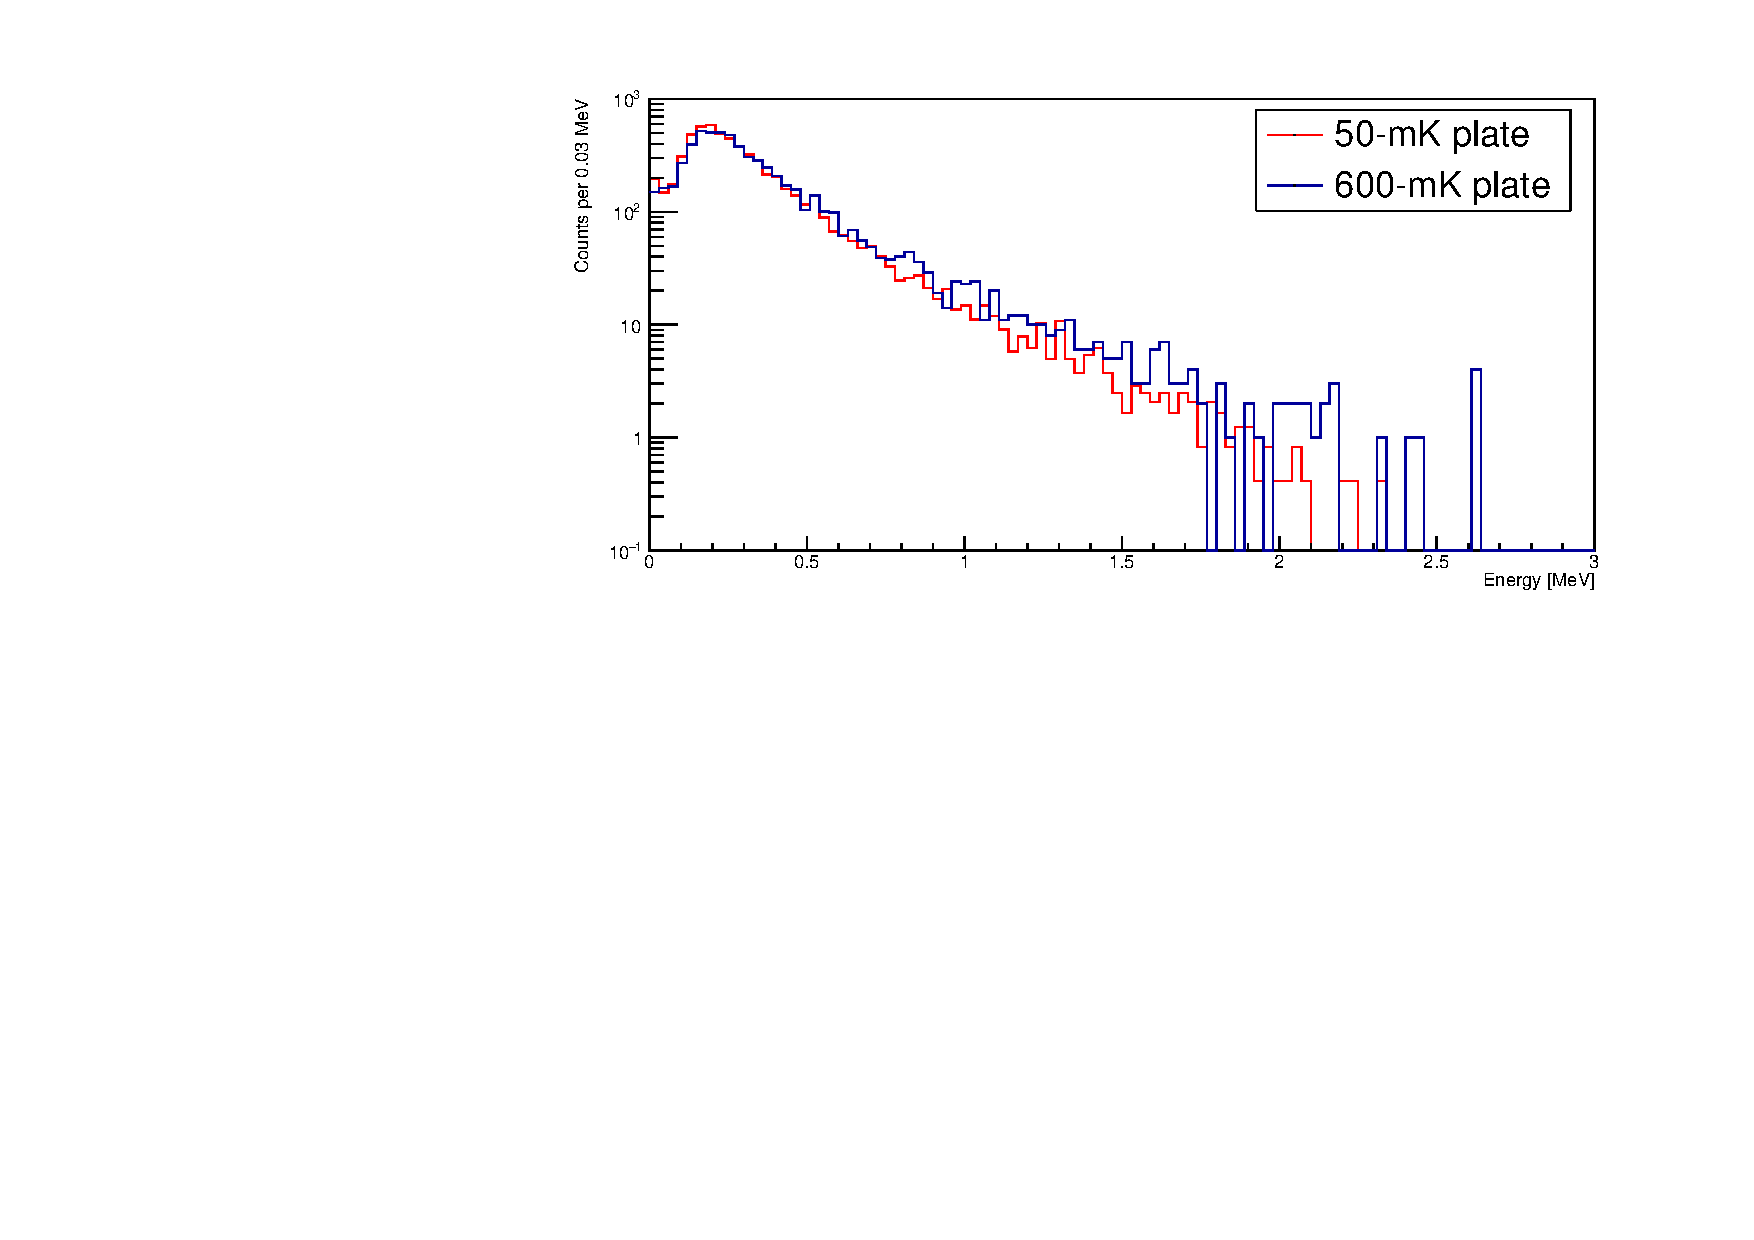
\includegraphics[width=0.8\linewidth]{Figures/th232_copper_plates.pdf}
    \caption[Simulated rates from a $^{232}$Th source on the 50-mK and 600-mK plates.]
    {Simulated rates from a $^{232}$Th source on the 50-mK and 600-mK plates.
    The y-axis is arbitrary and the number of entries is normalized.
    The spectra produced by these two materials are nearly identical and are indistinguishable for performing a fit.}
    \label{fig:degenerate_sources}
\end{figure}
In this way, much of the complexity of the fit can be reduced by combining sources as many cryostat components produce similar energy spectra for various contaminations, particularly for elements such as the copper vessels which are composed of the same material and are expected to have similar contaminations.
While some of this degeneracy could be removed by including the complete position information in the fit, only information on the general position of the incident radiation is included in the fit as the information from $\approx1000$ crystals would add significantly more free parameters, require a similar increase in the computation time to generate simulated spectra for each crystal, and further split the limited statistics by the same factor.

However, this position information for the sources can be a strong indicator for asymmetric sources in the cryostat.
For example, in CUORE-0, an excess of $^{232}$Th and $^{40}$K events on some crystals were determined to be due to spot sources on the 50-mK shield and the bottom of the external lead shield.
While CUORE benefits from improved procedures for handling and cleaning materials, it is not unreasonable to expect that there may be similar situations on CUORE, and indeed, excesses are observed in the data, as shown in \autoref{fig:k40_towers}, \autoref{fig:k40_towerfloors}, \autoref{fig:Co60_towers}, and \autoref{fig:po210_towers}.

\begin{figure}
    \centering
    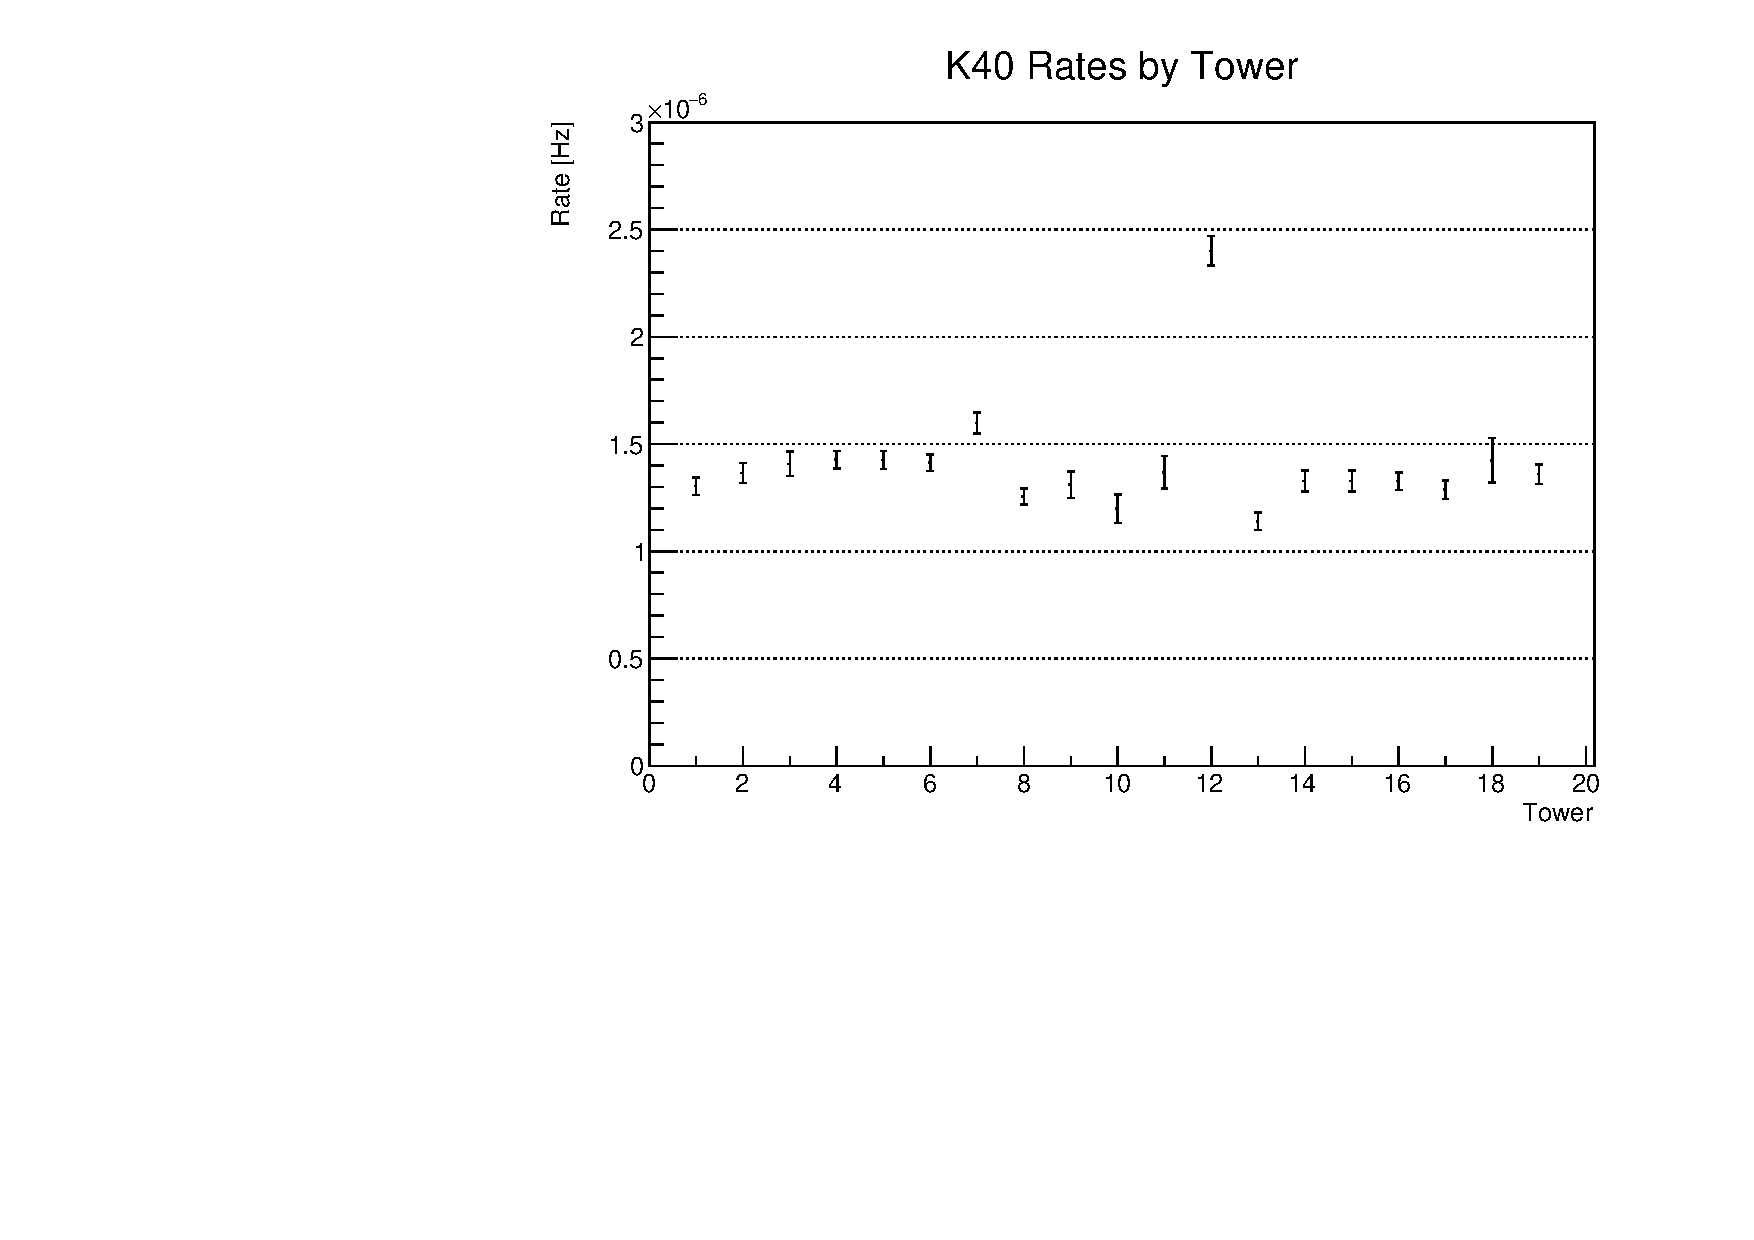
\includegraphics[width=0.8\linewidth]{Figures/K40AllTowers.pdf}
    \caption[The rate of $^{40}$K $\gamma$ events on each CUORE tower.]
    {The rate of $^{40}$K $\gamma$ events on each CUORE tower.
    While nearly all the towers have similar rates, an excess is observed on tower 12.}
    \label{fig:k40_towers}
\end{figure}

\begin{figure}
    \centering
    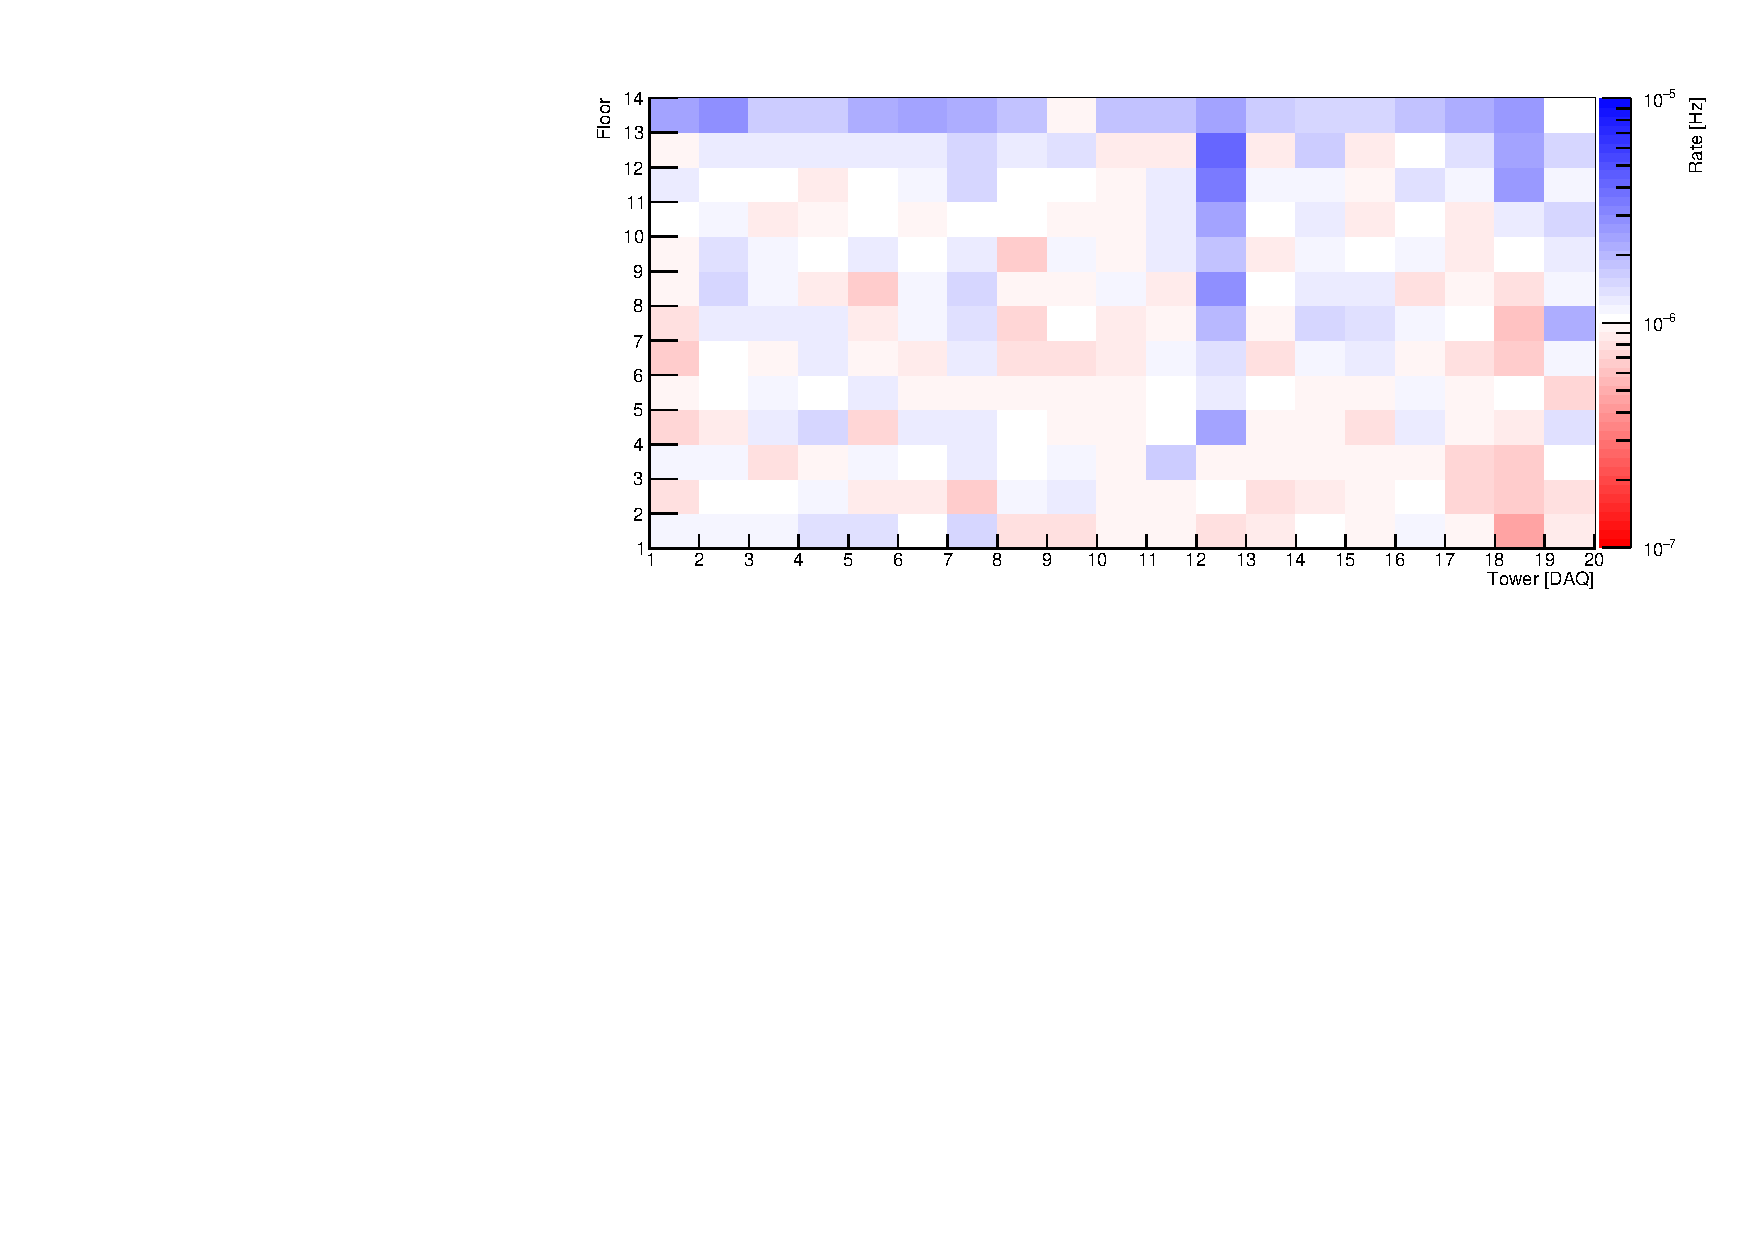
\includegraphics[width=0.9\linewidth]{Figures/K40TowerFloor.pdf}
    \caption[The rate of $^{40}$K $\gamma$ events on each CUORE tower, split into each floor.]
    {The rate of $^{40}$K $\gamma$ events on each CUORE tower, split into each floor.
    There are significantly higher rates along the top floor of each tower, and along many of the floors on tower 12.}
    \label{fig:k40_towerfloors}
\end{figure}

\begin{figure}
    \centering
    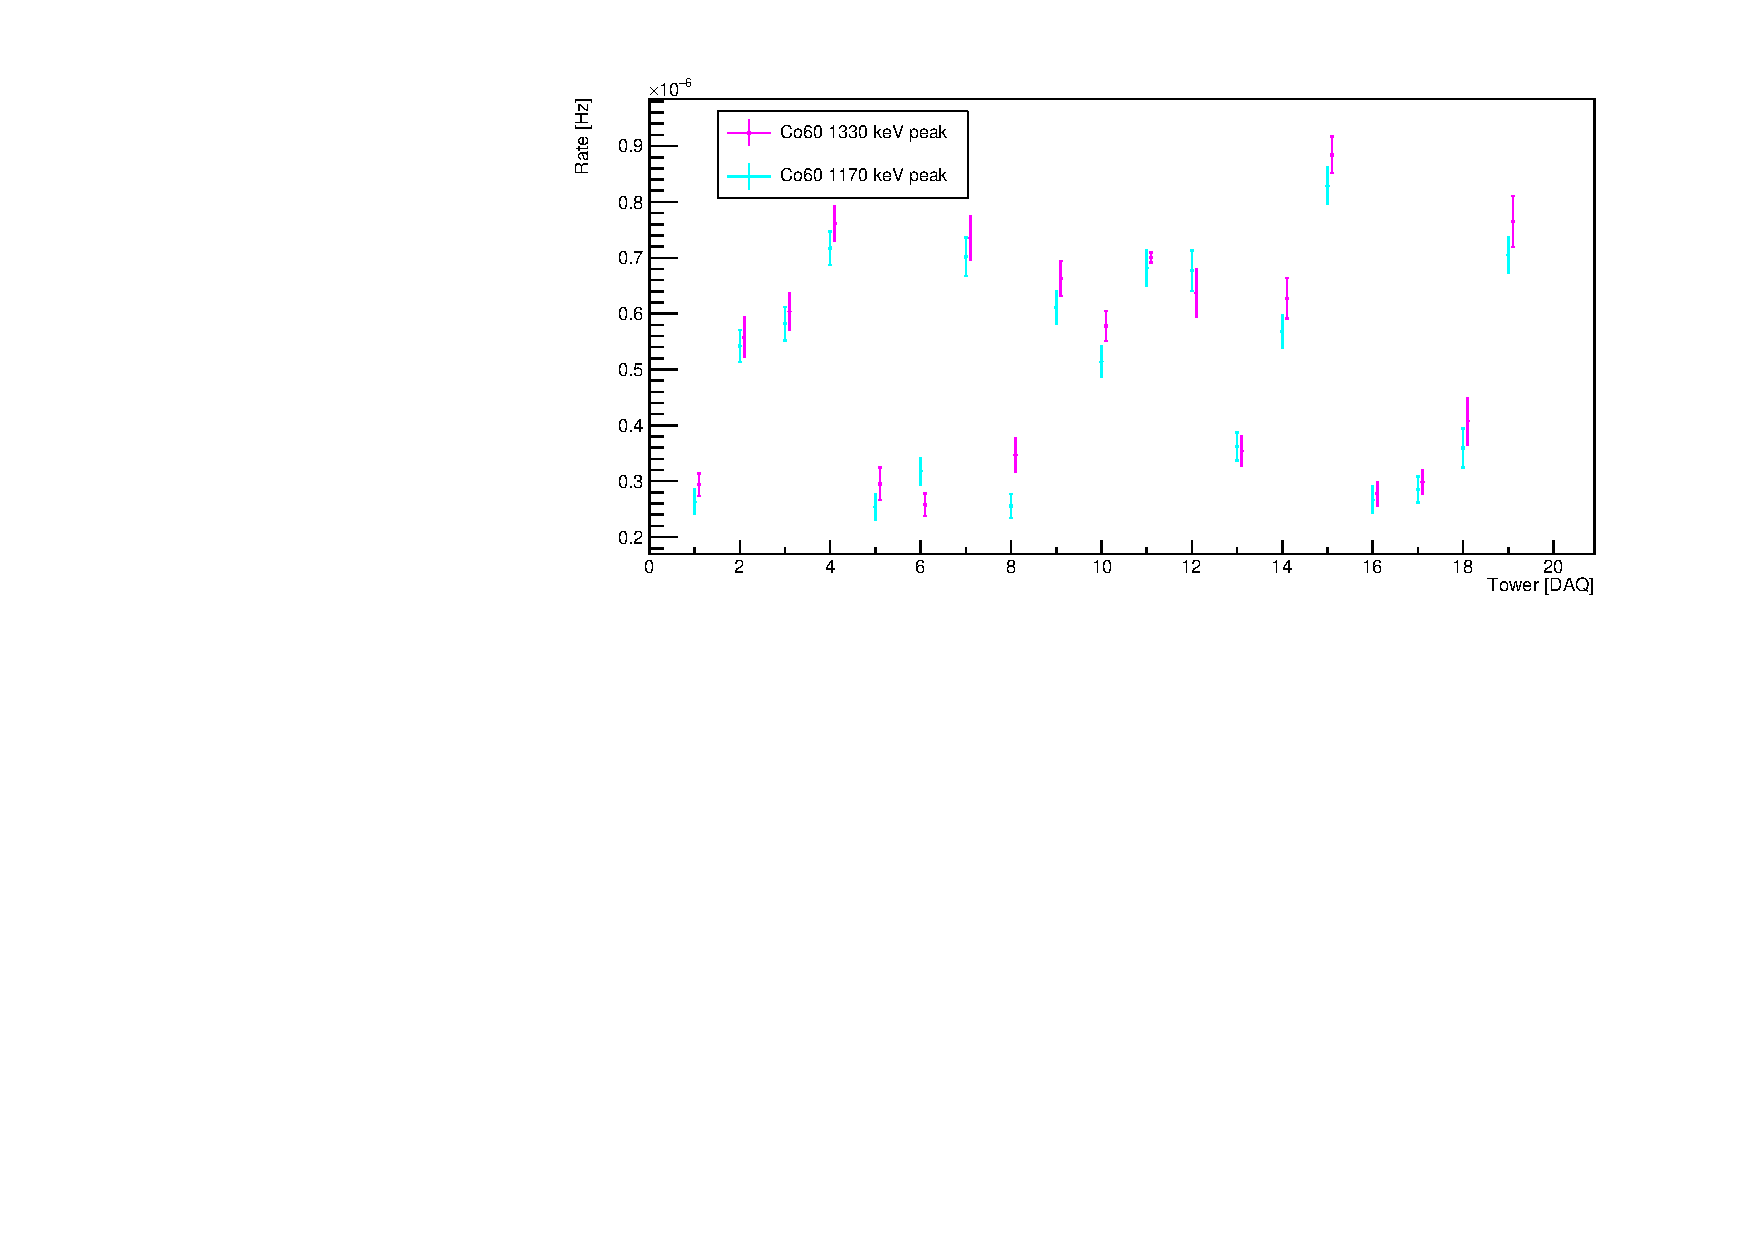
\includegraphics[width=0.8\linewidth]{Figures/Co60_combined.pdf}
    \caption[The rates of Co-60 decays at the 1330 and 1170 keV peaks.]
    {The rates of Co-60 decays at the 1330 and 1170 keV peaks.
    These events occur in coincidence at nearly equal rates during the decay of $^{60}$Co to $^{60}$Ni and the observed rates are consistent.
    Note that the 1330 keV peak is shifted rightwards along the x-direction by 0.1 for clarity.}
    \label{fig:Co60_towers}
\end{figure}

\begin{figure}
    \centering
    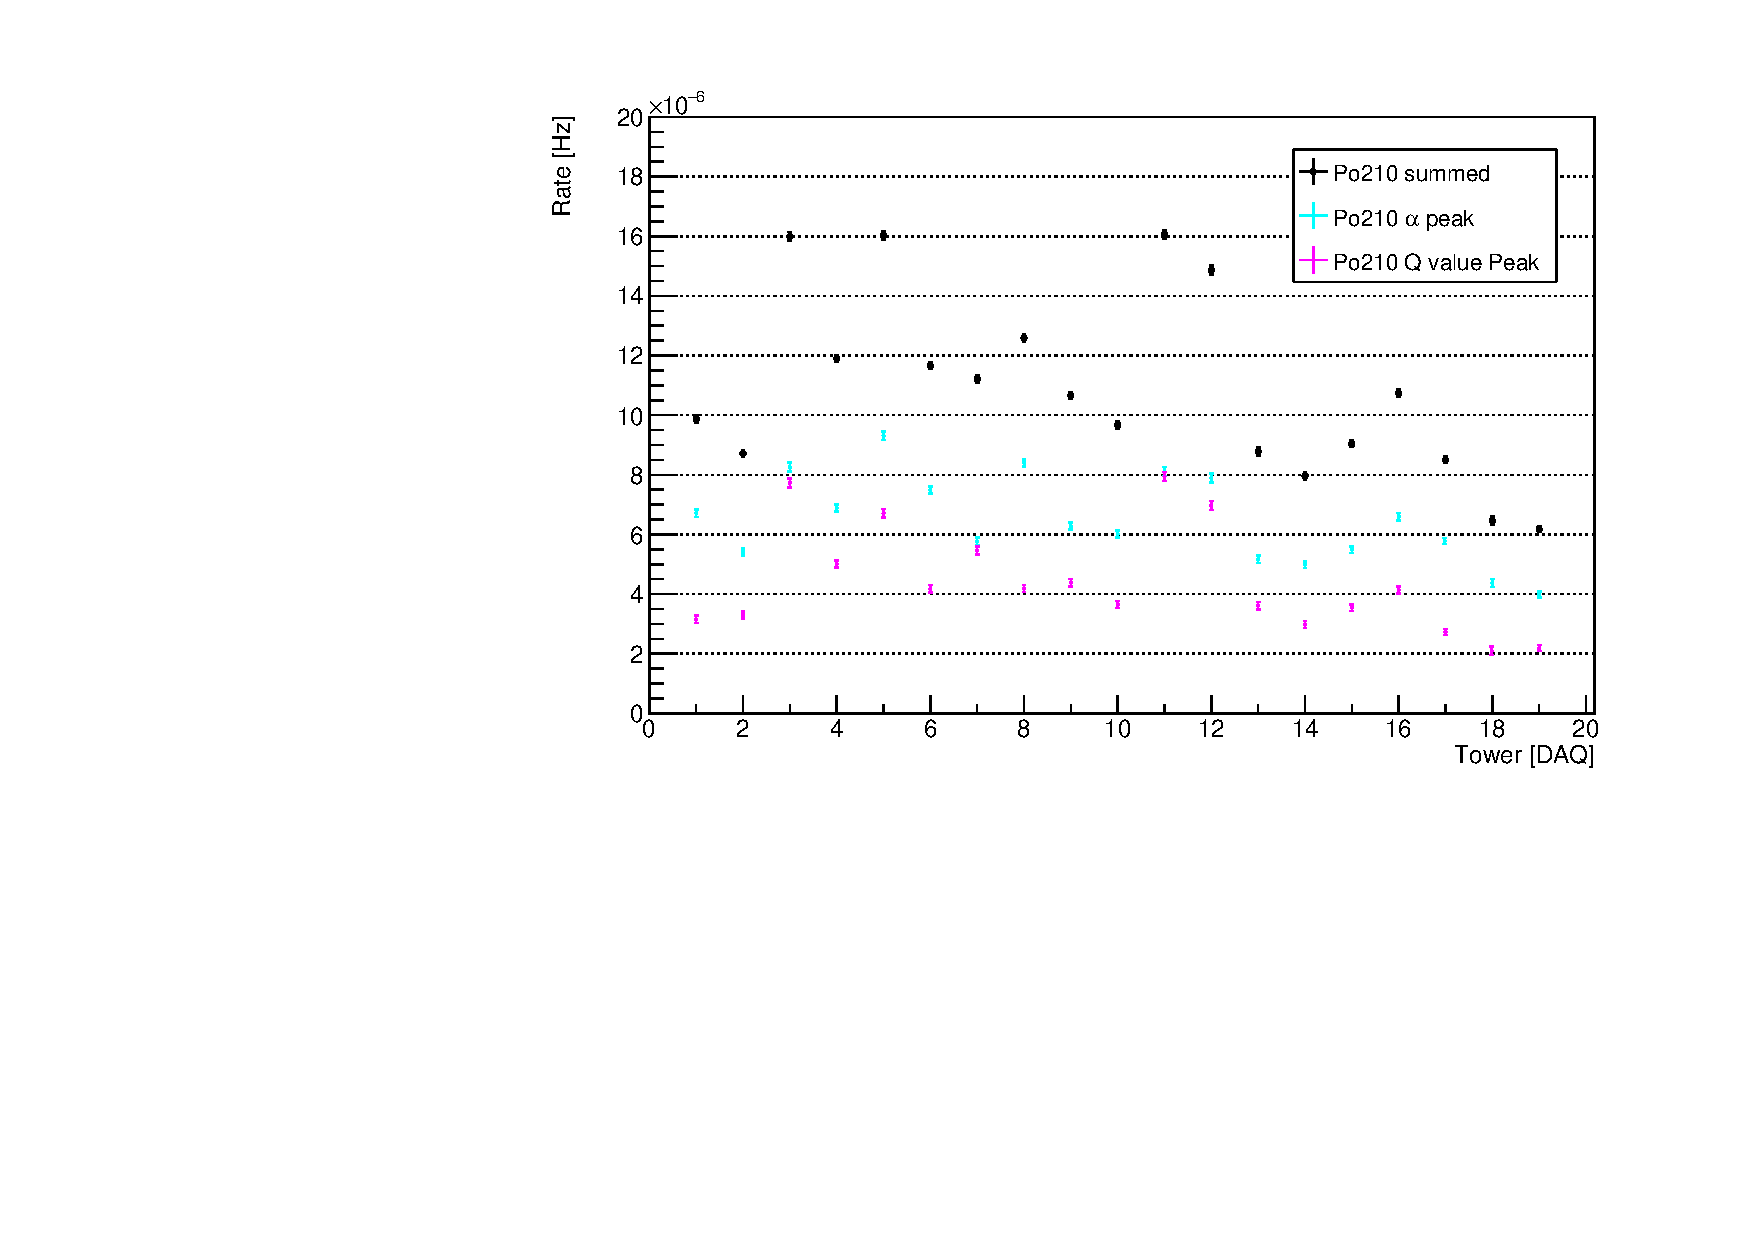
\includegraphics[width=0.8\linewidth]{Figures/Po210AllTowers.pdf}
    \caption[The rates of the Po-210 contaminations on the towers including the Q-value and $\alpha$ peaks.]
    {The rates of the Po-210 contaminations on the towers including the Q-value and $\alpha$ peaks.
    There is significant spread in the Po-210 rates along the towers, likely corresponding to the age of the towers ($T_{1/2}=$138 days) and contaminations during crystal growth.}
    \label{fig:po210_towers}
\end{figure}

Unfortunately, many of these studies of these sources are currently statistics-limited, and CUORE lacks the data to perform a full analysis to characterize each of these asymmetric background sources.
For example, with a year of live-time, a 1 $\mu$Hz rate on a channel corresponds to merely approximately 30 expected events.
Therefore, for now with the \livetime~of data in CUORE, there are a few candidates that are apparent, such as the excess of $^{40}$K events on tower 12, but precisely defining and locating these exact sources remains out of reach at present.
That said, while a fully complete background model would include these sources, these geometrical differences can be treated as a systematic in the fits produced by the data.
This is achieved by selecting data according to various geometrical subsets of the data, e.g. by fitting only odd/even floors or by odd/even towers, since the rates for Majoron emission are independent of the particular tower geometry.

\subsubsection*{Creating the Background Model}

The sum of each of the background sources in CUORE forms the background model of the experiment.
The model can be written as a sum of the normalizations of each of the $N$ Monte Carlo spectra as
\begin{align}
    B_\alpha &= \sum_j^N C_{j} \cdot M_{j,\alpha} 
\end{align}
where the $B_{\alpha}$ is the background model for the data splitting $\alpha$\footnote{Generally speaking, this splitting is typically done according to the multiplicity, viz. M1, M2, etc. spectra, but can also include other splittings as well.}, $C_{j}$ is the normalization factor for the $j^{\textrm{th}}$ simulated spectra, and similarly $M_{j,\alpha}$ is the number of counts in the $j^{\textrm{th}}$ simulated spectrum for the same multiplicity $\alpha$.
In a Bayesian approach, the goal of creating the background model is to then define a joint posterior probability distribution funciton defined by
\begin{align}
\begin{split}
        Posterior(C_j, \langle M_{j,\alpha}\rangle|B_\alpha, M_{j,\alpha}) = \prod_\alpha Poisson(B_\alpha|\langle B_\alpha\rangle)\times \prod_j Prior(C_j) \\ \times \prod_{j, \alpha}Poisson(M_{j,\alpha}|\langle M_{j,\alpha}\rangle) \times Prior(\langle M_{j,\alpha}\rangle)
\end{split}
\end{align}
where $\langle x \rangle$ is the expectation value of $x$, $Poisson(x|y)$ is the Poisson probability of observing $x$ with mean $y$, and $Prior(x)$ is the prior distribution of $x$.
This somewhat intimidating posterior is merely just a rewriting of Bayes' theorem, given that both the real and simulated data both obey Poisson statistics and that a prior is included on each of these parameters.
Of course, in Bayesian statistics, everything comes down to the choice of priors\footnote{\RaggedRight A cute caricature of which is described here: \url{https://xkcd.com/1132/}}.
As discussed in \autoref{ssec:Parts Selection and Cleaning} and \autoref{ssec:Cryostat_Radiopurity}, these measurements of background activity in the fit could begin to constrain a few of the priors for $C_j$ used, but, even with upper limits, a choice needs to be made about the form of these priors.
For this analysis then, the form for these priors is chosen to be a uniform non-informative prior that covers a large range from 0\footnote{Naturally, having a contribution produce a negative addition to the spectrum is unphysical, but this can introduce a slight positive fit bias.} to a significant overestimation of the contribution to the background model.
Lastly, this background model is, in order to simplify the fitting and to reduce the effect of other systematics, treated as a binned analysis with varying bin size.
In particular, while the bin size is set to a minimum width of 15 keV, the regions around each $\gamma$ or $\alpha$ peak are merged into a single bin in order to remove systematic uncertainties due to the particular shape of the peak, and, in addition, bins with $<30$ counts are also merged to reduce the effect of statistical fluctuations.
In addition, this bin size also sets the maximum range on each of the uniform priors.
This is done by assuming that a particular source contributes every count in a bin, and the upper limit on the prior is set to be twice the maximum normalization $C_j$ that satisfies this.
\begin{table}[htbp]
    \centering
    \caption[The background model components for CUORE]
    {The background model components for CUORE.
    The surface contaminations are modeled at multiple depths as some sources exhibit differing spectra at shallower or deeper depths. \color{red}Add Sm-147?\color{black}}
    \label{tab:background_model_list}
\begin{tabular}{l|l|l}
\hline
\hline
Volume  & Type & Components \\
\hline
\multirow{2}{*}{TeO$_2$} & \multirow{2}{*}{Bulk} & $2\nu\beta\beta$, $^{210}$Pb, $^{232}$Th, $^{228}$Ra - $^{208}$Pb, $^{238}$U-$^{230}$Th, \\
 & & $^{230}$Th, $^{226}$Ra-$^{210}$Pb, $^{40}$K, $^{60}$Co $^{125}$Sb, $^{190}$Pt \\
 \hline
\multirow{3}{*}{TeO$_2$} & Surface (0.01\mu m) & $^{232}$Th, $^{228}$Ra - $^{208}$Pb, $^{238}$U-$^{230}$Th, $^{226}$Ra-$^{210}$Pb, $^{210}$Pb \\
        & Surface (1~$\mu$m) & $^{210}$Pb \\
        & Surface (10~$\mu$m) & $^{210}$Pb, $^{232}$Th, $^{238}$U \\
\hline
CuNOSV & Bulk & $^{232}$Th, $^{238}$U, $^{40}$K, $^{60}$Co, $^{40}$Mn \\
\hline
\multirow{3}{*}{CuNOSV}& Surface (0.01 $\mu$m) & $^{210}$Pb, $^{232}$Th, $^{238}$U \\
    & Surface (1 $\mu$m) & $^{210}$Pb, $^{232}$Th, $^{238}$U \\
    & Surface (10 $\mu$m) & $^{210}$Pb, $^{232}$Th, $^{238}$U \\
\hline
Roman Lead & Bulk & $^{232}$Th, $^{238}$U, $^{108m}$Ag \\
Top Lead & Bulk & $^{232}$Th, $^{238}$U, $^{210}$Bi \\
Ext Lead & Bulk & $^{210}$Bi \\ 
\hline
CuOFE & Bulk & $^{232}$Th, $^{238}$U, $^{60}$Co \\
\hline
External & & Cosmic $\mu$ \\
\hline
\hline
\end{tabular}
\end{table}

\section{Markov Chain Monte Carlo}
\label{sec:MCMC}
Performing a simultaneous fit of $60+$ spectra is a non-trivial challenge, particularly as each component to the fit is generally composed of a spectrum that can span a range from a few keV up to multiple MeV. 
However, Markov Chain Monte Carlo provides a tractable solution to this computationally difficult multidimensional fit.
This method can be thought of as performing a random walk\footnote{The Gibbs Sampling technique used in this work does not perform a random walk in the traditional sense.
Namely, every time a new step determines an improved $\chi^2$, the new value is sampled, as opposed to other MCMC methods where the step would only be taken in a probabilistic manner.} in the available parameter space that minimizes a likelihood estimator such as the standard
\begin{equation}
\label{eq:chi_squared}
\chi^2=\sum_i \frac{(O_i-E_i)^2}{E_i}
\end{equation}
likelihood, where $O_i$ and $E_i$ are the observed and expected counts in the $i^{\textrm{th}}$ bin.
This random walk then samples the joint posterior probability distribution function of the model parameters of the MCMC.

To perform this MCMC fit, we use a program called Just Another Gibbs Sampler (JAGS)\footnote{\RaggedRight\url{http://mcmc-jags.sourceforge.net/}}.
Gibbs sampling, for which this program is named, uses a simple procedure to fit the spectra:
\begin{enumerate}
    \item Choose an arbitrary value of each $C_j^{(0)}$
    \item Update each normalization $C_j^{(i+1)}$ from the distribution one at a time, holding the others constant and storing the history of each $C_j^{(i)}$
    \begin{itemize}
        \item Update $C_1^{(i+1)}$ from by fitting the data, D, with all other normalizations held fixed, namely, $\theta(C_1^{(i+1)}|C_2^{(i)}, ..., C_N^{(i)}, D)$
        \item Update $C_2^{(i+1)}$ with $\theta(C_2^{(i+1)}|C_1^{(i+1)}, C_3^{(i)}, ..., C_N^{(i)}, D)$
        \item ...
        \item Update $C_N^{(i+1)}$ with $\theta(C_N^{(i+1)}|C_1^{(i+1)}, ..., C_{N-1}^{(i+1)}, D)$
    \end{itemize}
    \item Lastly, once enough samples are generated, finish the procedure, else continue with step 2
\end{enumerate}
Bias introduced due to the guess of the initial conditions for $C_j$ can be minimized through a technique called ``burn-in" where the first initial steps of the MCMC are discarded and thrown away.
As the number of MCMC steps goes to infinity, the full parameter space will be walked irrespective of the initial conditions set, but, given computing limitations, this burn-in time allows for the MCMC to walk around from the initial conditions towards a more ``natural" set of parameters\footnote{Consider the case where the initial conditions set normalization constants at the highest end of their priors when the ``true" contribution of the spectrum is 0.
The MCMC will walk away from these points quickly, but the regions of parameter space near the initial conditions will be oversampled, introducing bias.}
In addition, another source of bias is through autocorrelation errors.
As listed above, each set of parameters $C_j^{(i)}$ depends on the previous set of parameters $C_j^{(i-1)}$, which introduces this autocorrelation, but can be dealt with by means of a technique called ``thinning".
With this technique, the samples of the MCMC are only recorded for every k$^{\textrm{th}}$ step with every $k-1$ steps thrown out.
While this causes large losses in efficiency, this benefits the MCMC results by reducing the effects of this bias\footnote{There are other MCMC techniques such as Hamiltonian MCMC that have the potential to avoid this ``thinning" solution and can more efficiently converge with less burn-in \cite{2017arXiv170102434B}.
These techniques are not used in this analysis, but could be used in future analyses.}.
\section{Majoron Analysis}
When fitting the data with JAGS, the spectrum is split into three main components: the single-crystal \Mone~spectrum, the multi-crystal \Mtwo~spectrum, and the summed multi-crystal \Msum~spectrum.
This is done as the signal events from a Majoron search mostly deposit energy into a single crystal, as is typical of events originating from the bulk of the crystal volume, whereas many other sources that are external to a crystal or on the surface have a higher probability of depositing energy into more than one crystal.
Higher multiplicity spectra are not used, as they do not add significant information to the fit for other sources.
The fit with the full background model, which will be called $H_0$, is shown in \color{red}include $H_0$ fit here\color{black}.
The $\chi^2$ of the fit is \color{red}insert $\chi^2$ here\color{black}.
For the fit, each of the possible Majoron spectral indices are considered independently and are shown for each multiplicity in \autoref{fig:SpectralIndicesM1Fit} and \autoref{fig:SpectralIndicesM2Fit}.

\begin{figure}[htbp]
\centering
\begin{subfigure}[t]{0.8\textwidth}
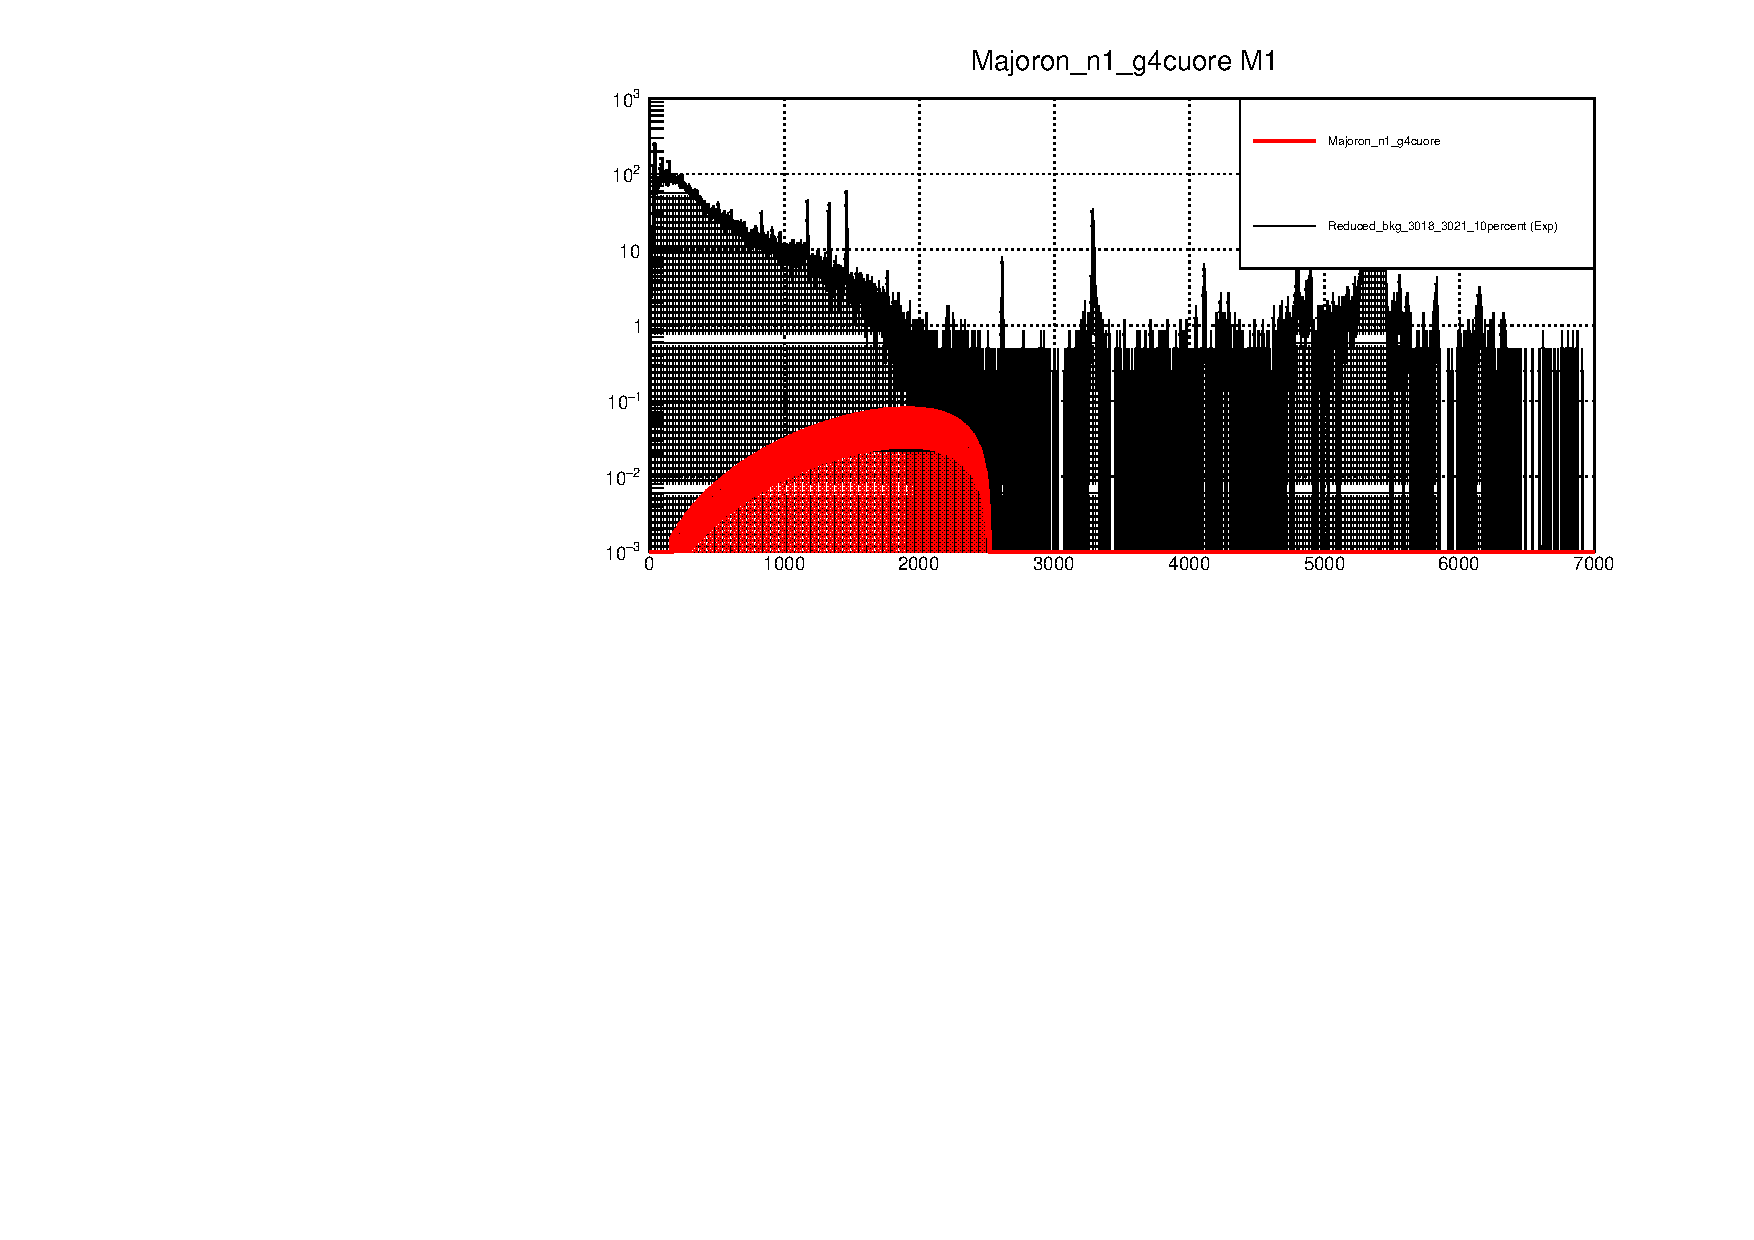
\includegraphics[width=0.9\textwidth]{Figures/Majoron_n1_g4cuore.pdf}
\end{subfigure}
\qquad
\begin{subfigure}[t]{0.8\textwidth}
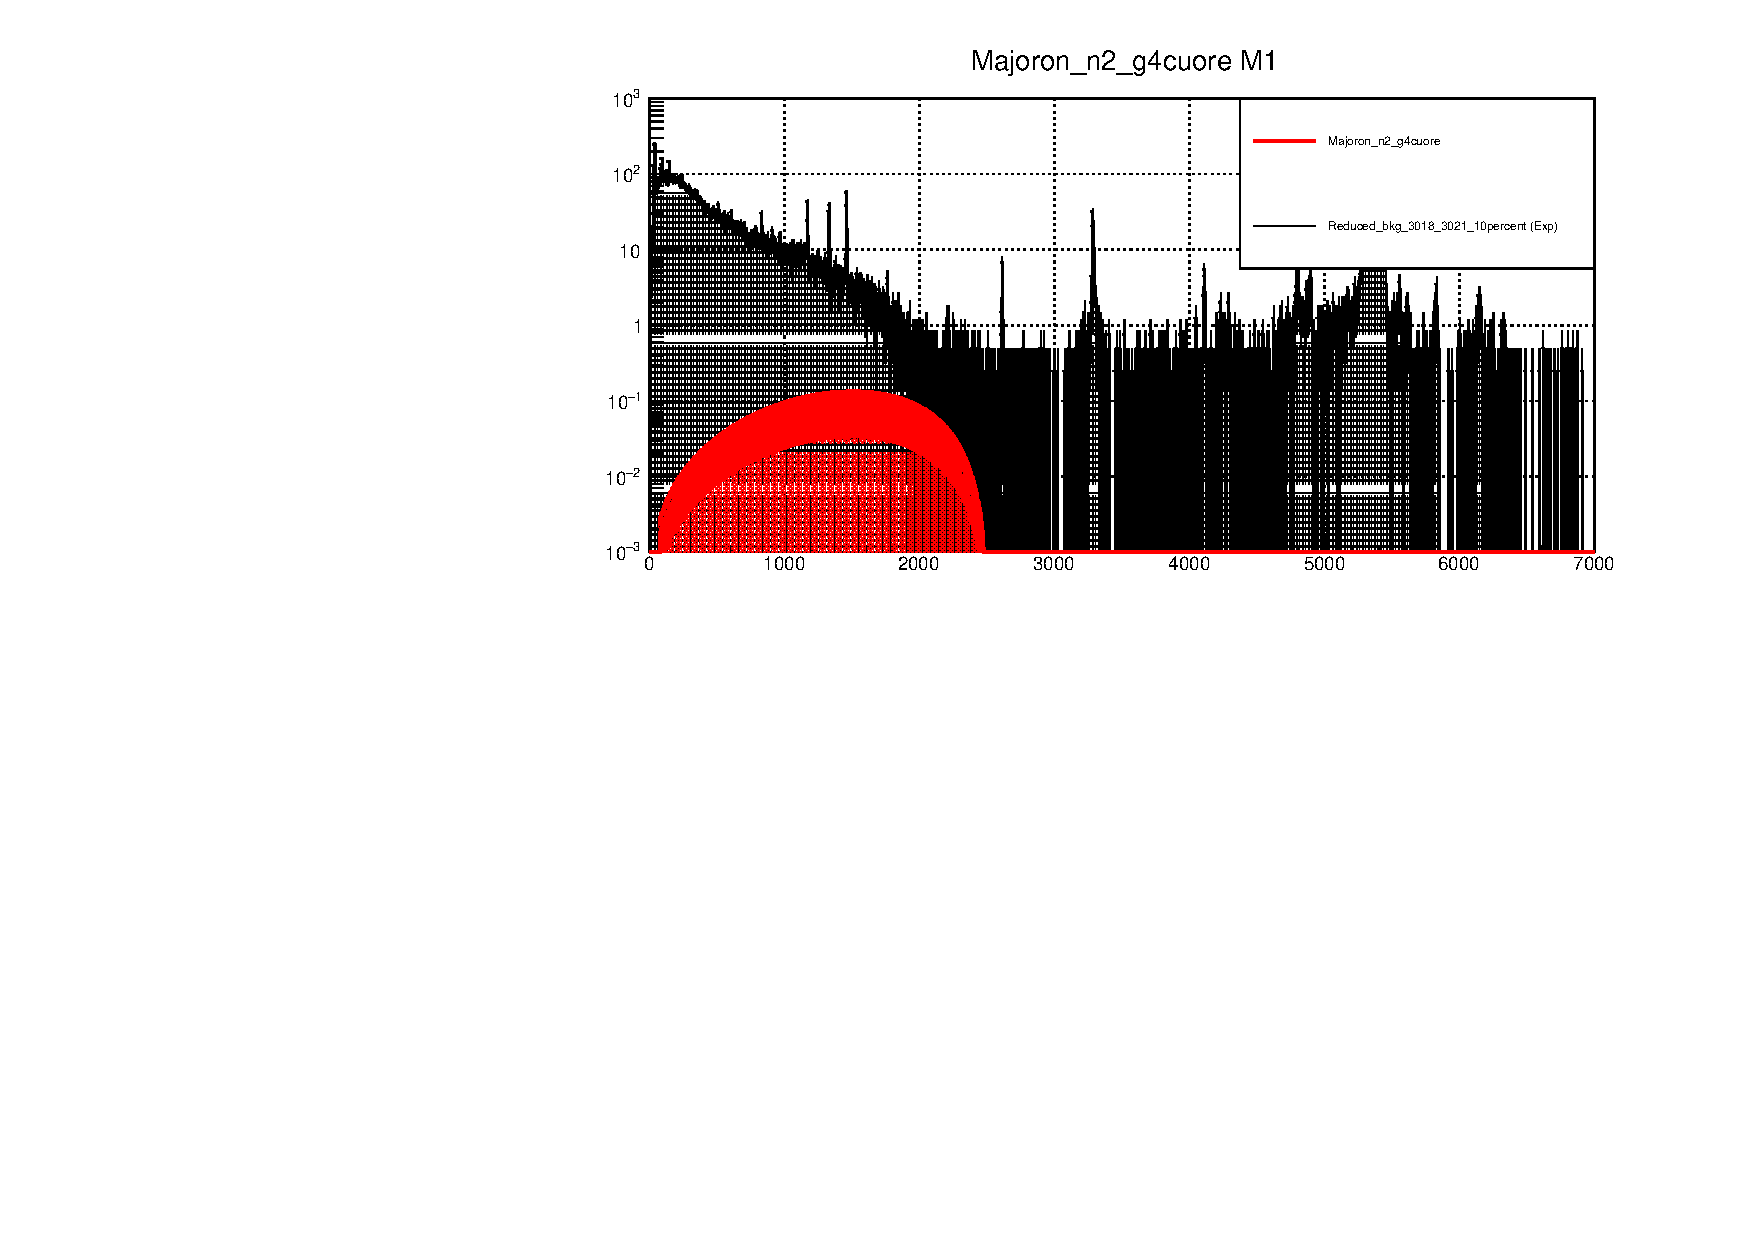
\includegraphics[width=0.9\textwidth]{Figures/Majoron_n2_g4cuore.pdf}
\end{subfigure}
\qquad
\begin{subfigure}[t]{0.8\linewidth}
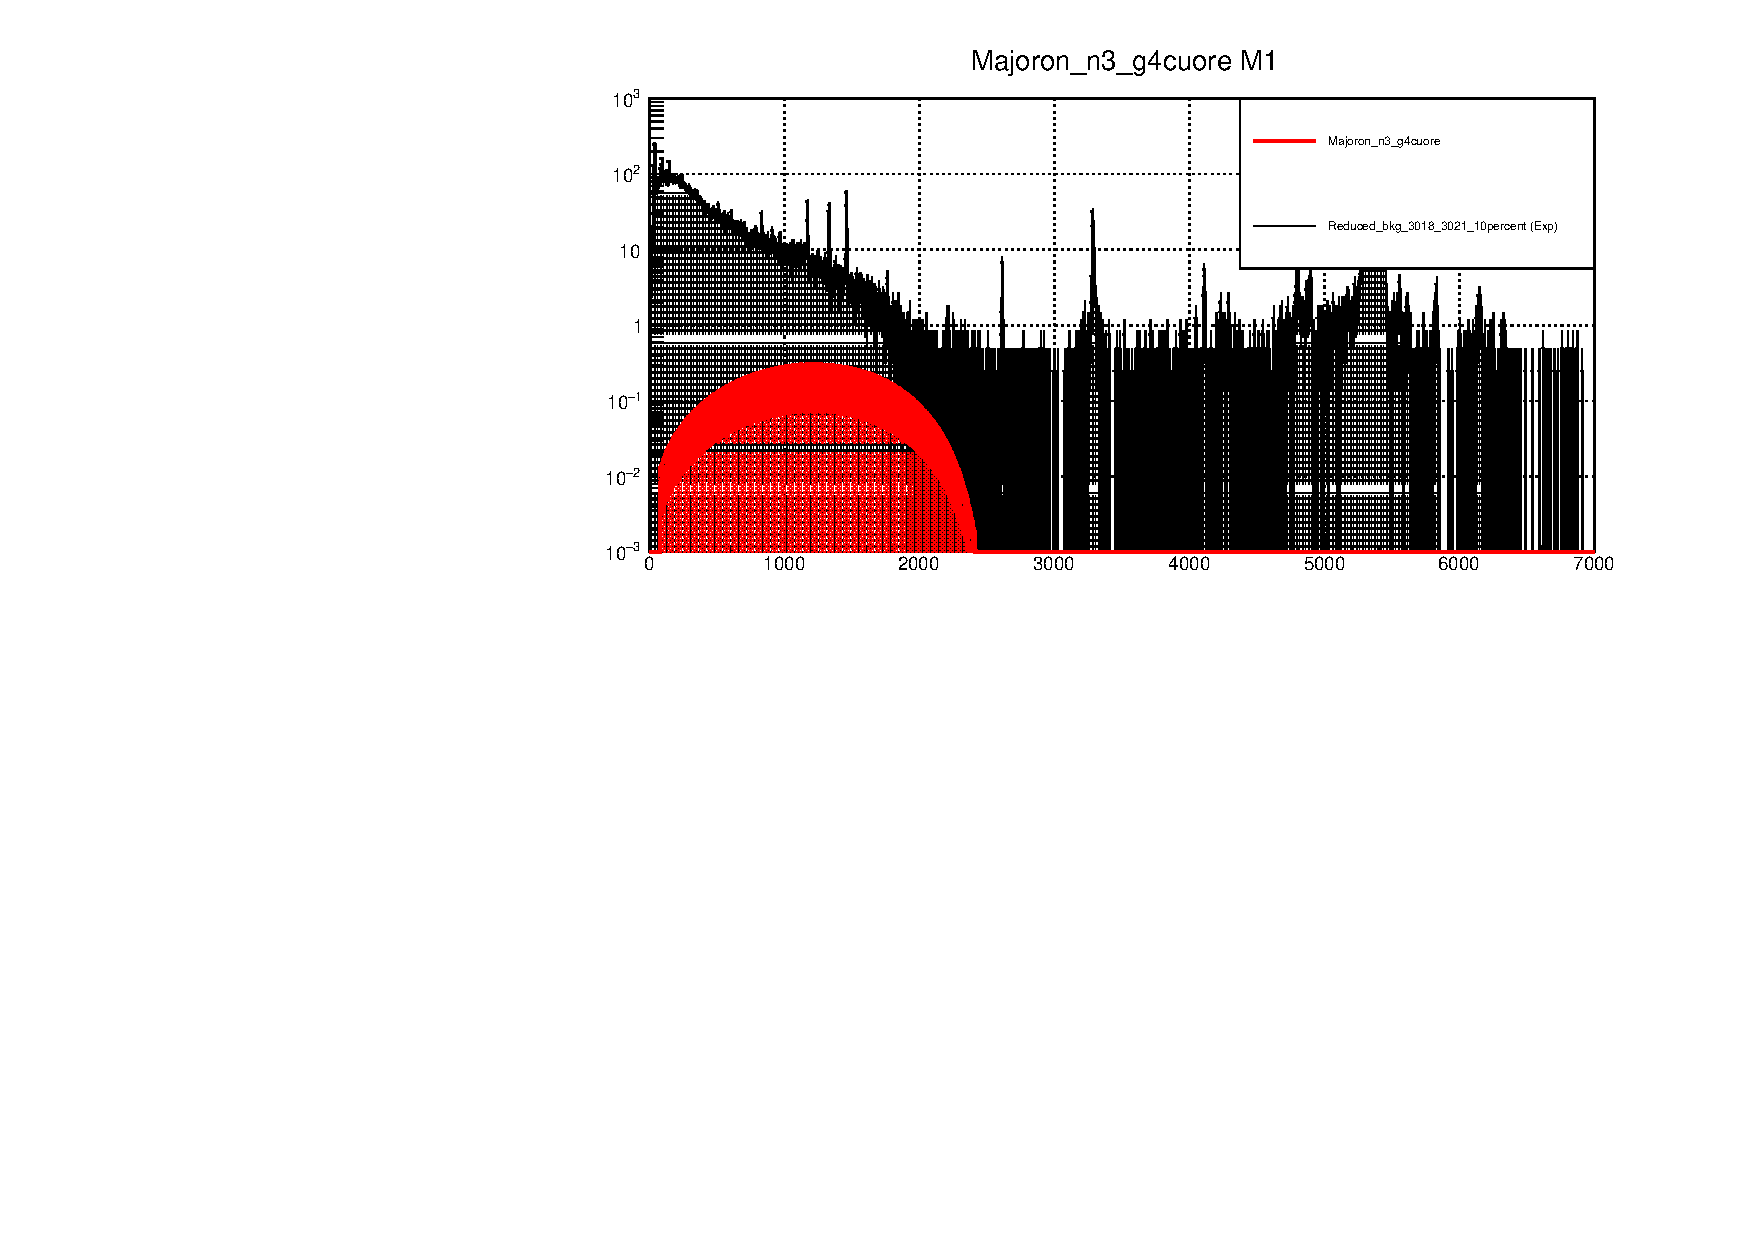
\includegraphics[width=0.9\textwidth]{Figures/Majoron_n3_g4cuore.pdf}
\end{subfigure}
\qquad
\begin{subfigure}[t]{0.8\linewidth}
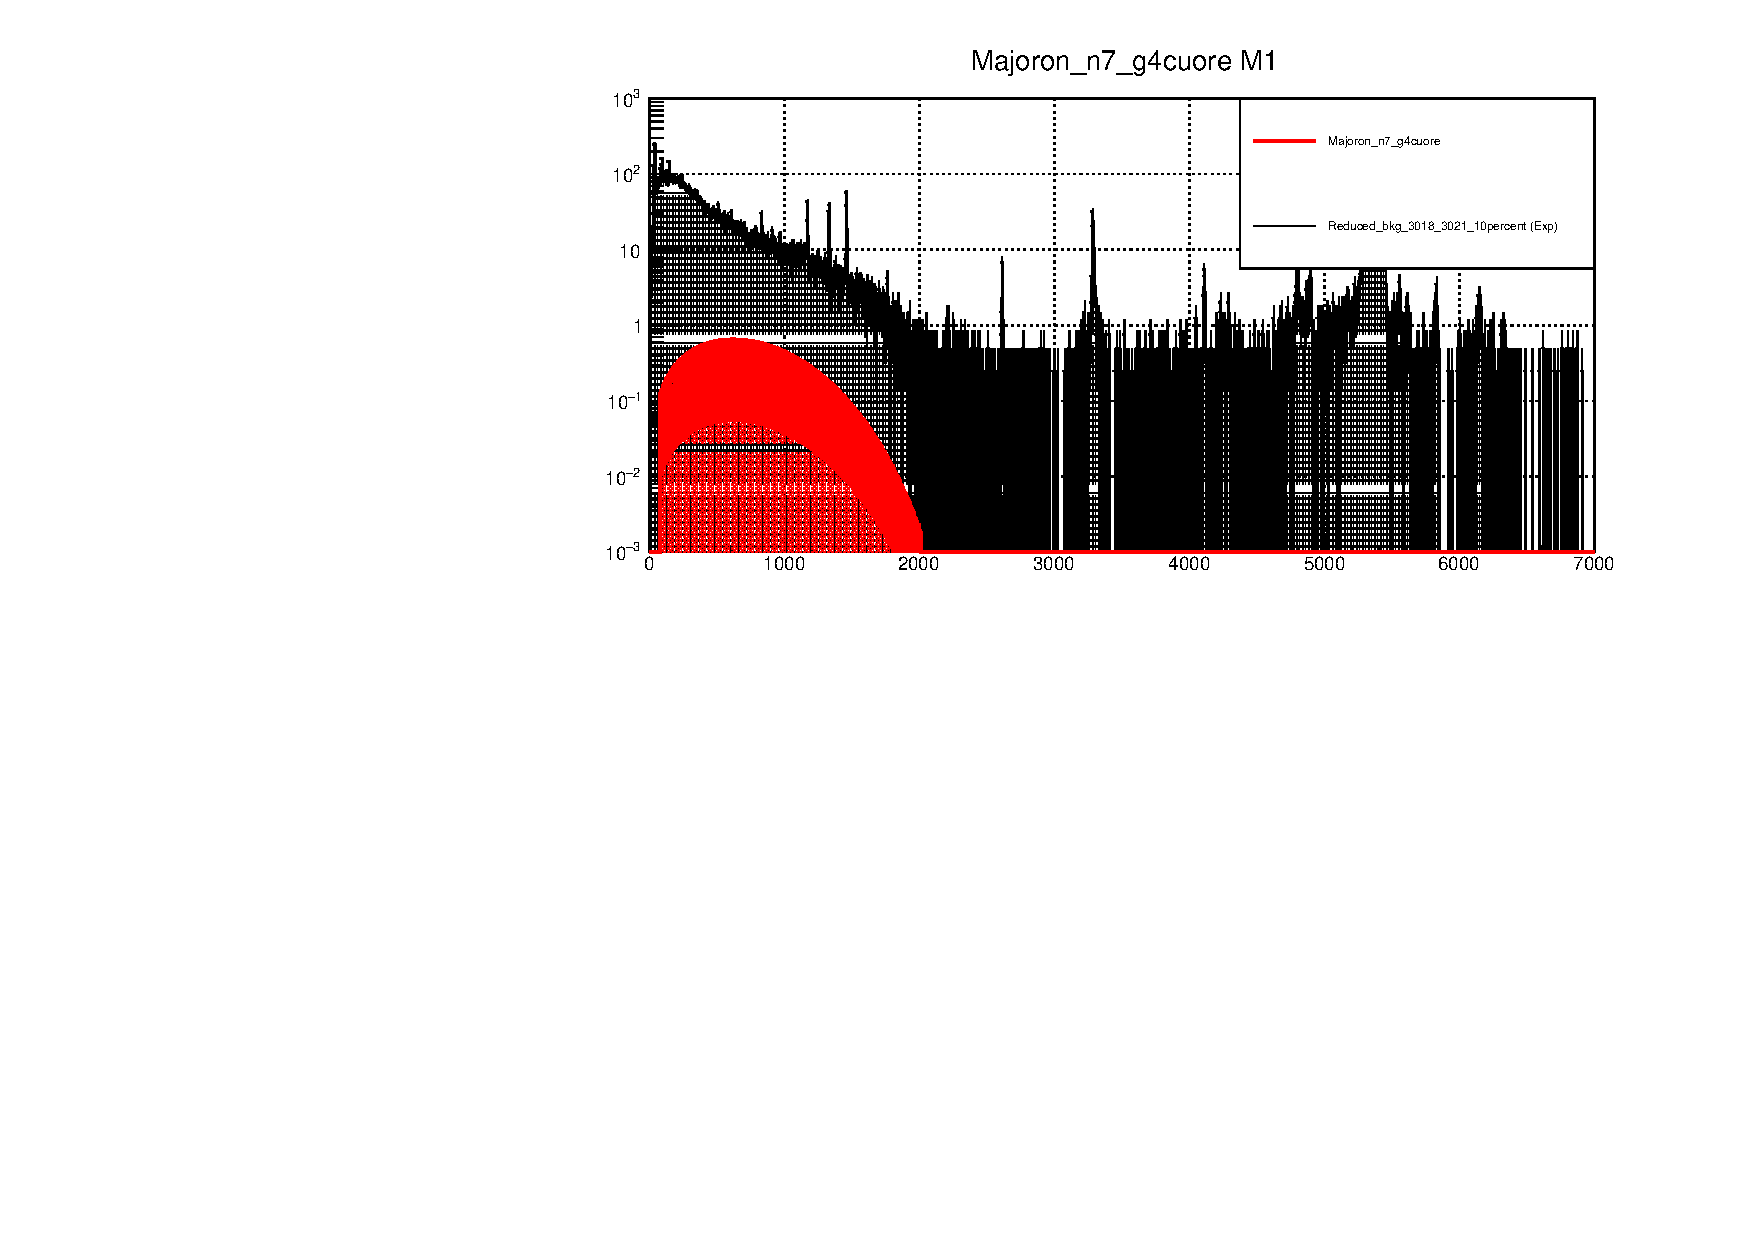
\includegraphics[width=0.9\textwidth]{Figures/Majoron_n7_g4cuore.pdf}
\end{subfigure}
\caption[The fitted contribution of Majoron decays for the different spectral indices in the \Mone~ spectrum]{The fitted contribution of Majoron decays for the different spectral indices in the \Mone~ spectrum.}
\label{fig:SpectralIndicesM1Fit}
\end{figure}

\begin{figure}[htbp]
\centering
\begin{subfigure}[t]{0.8\textwidth}
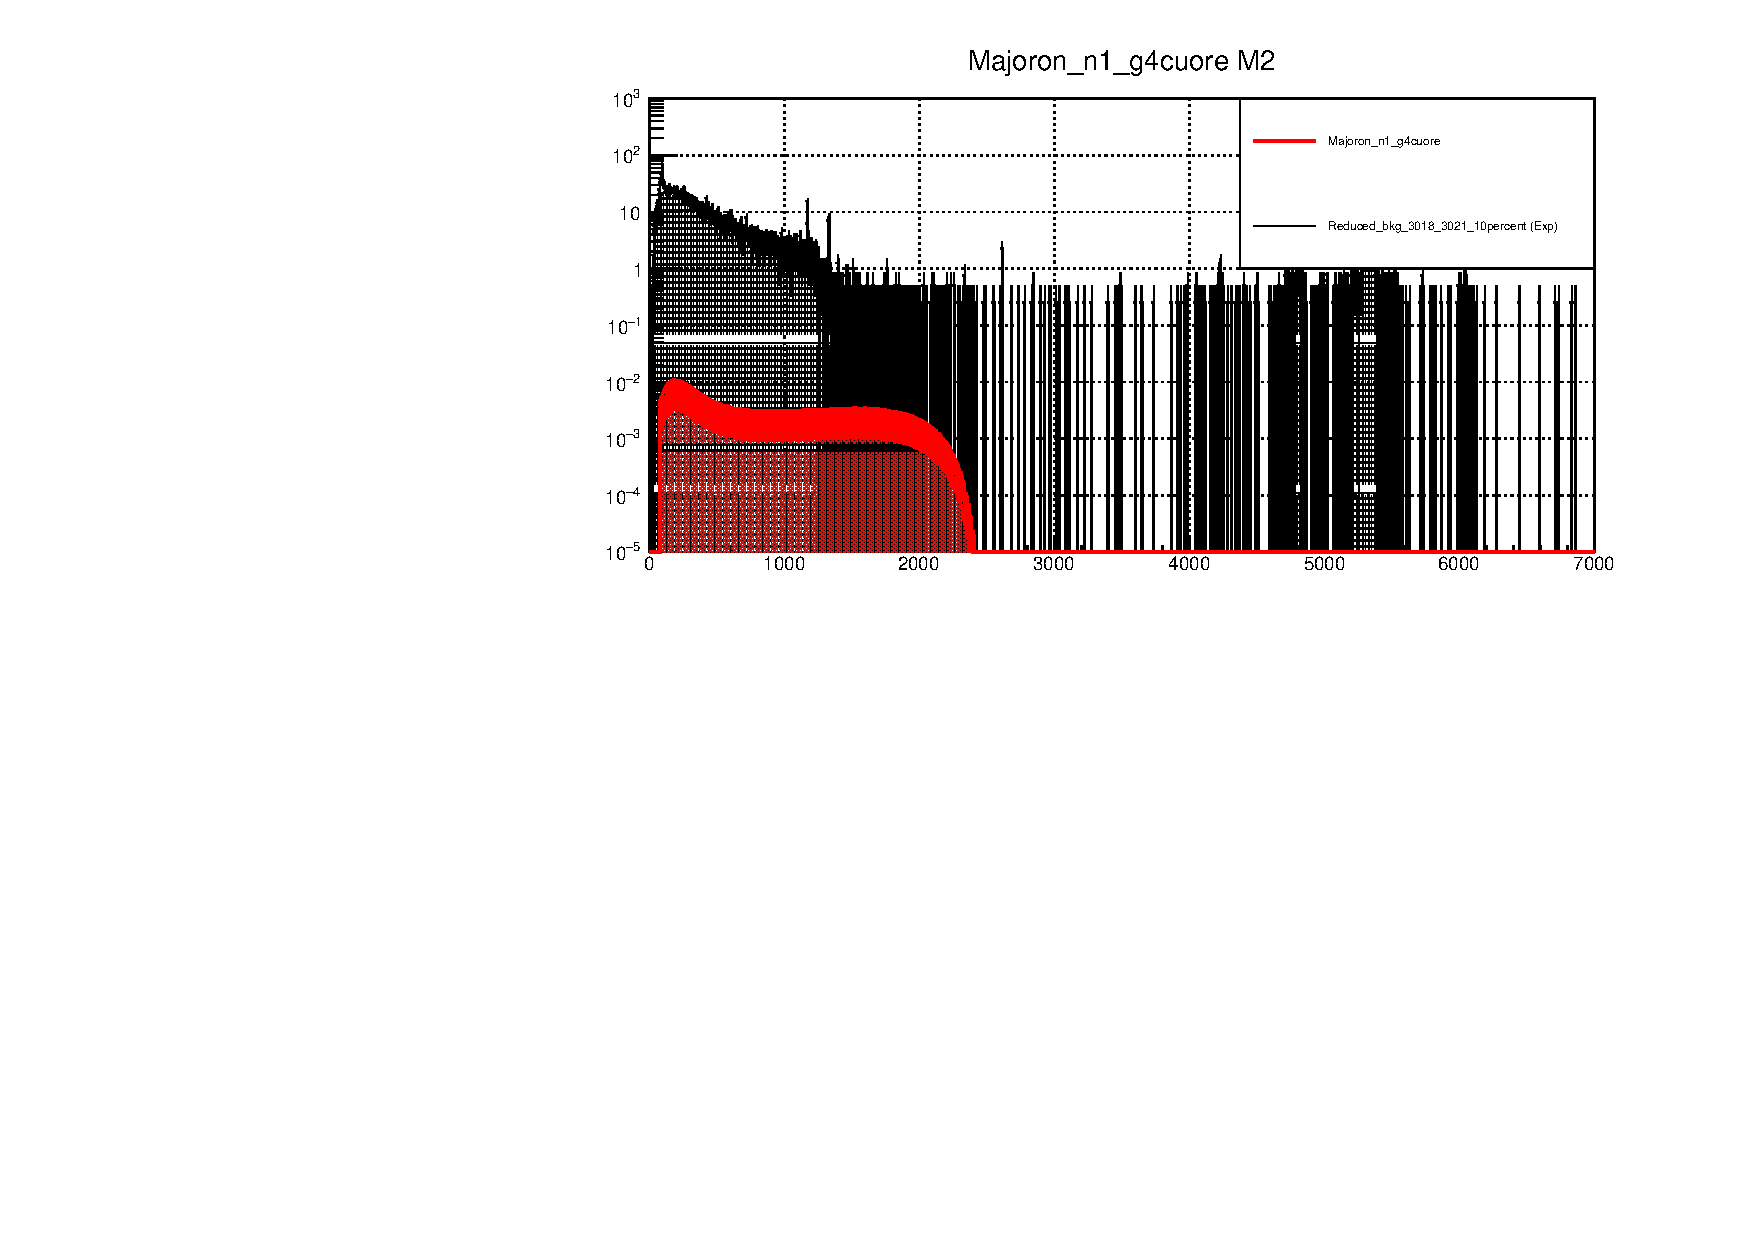
\includegraphics[width=0.9\textwidth]{Figures/Majoron_n1_g4cuore_M2.pdf}
\end{subfigure}
\qquad
\begin{subfigure}[t]{0.8\textwidth}
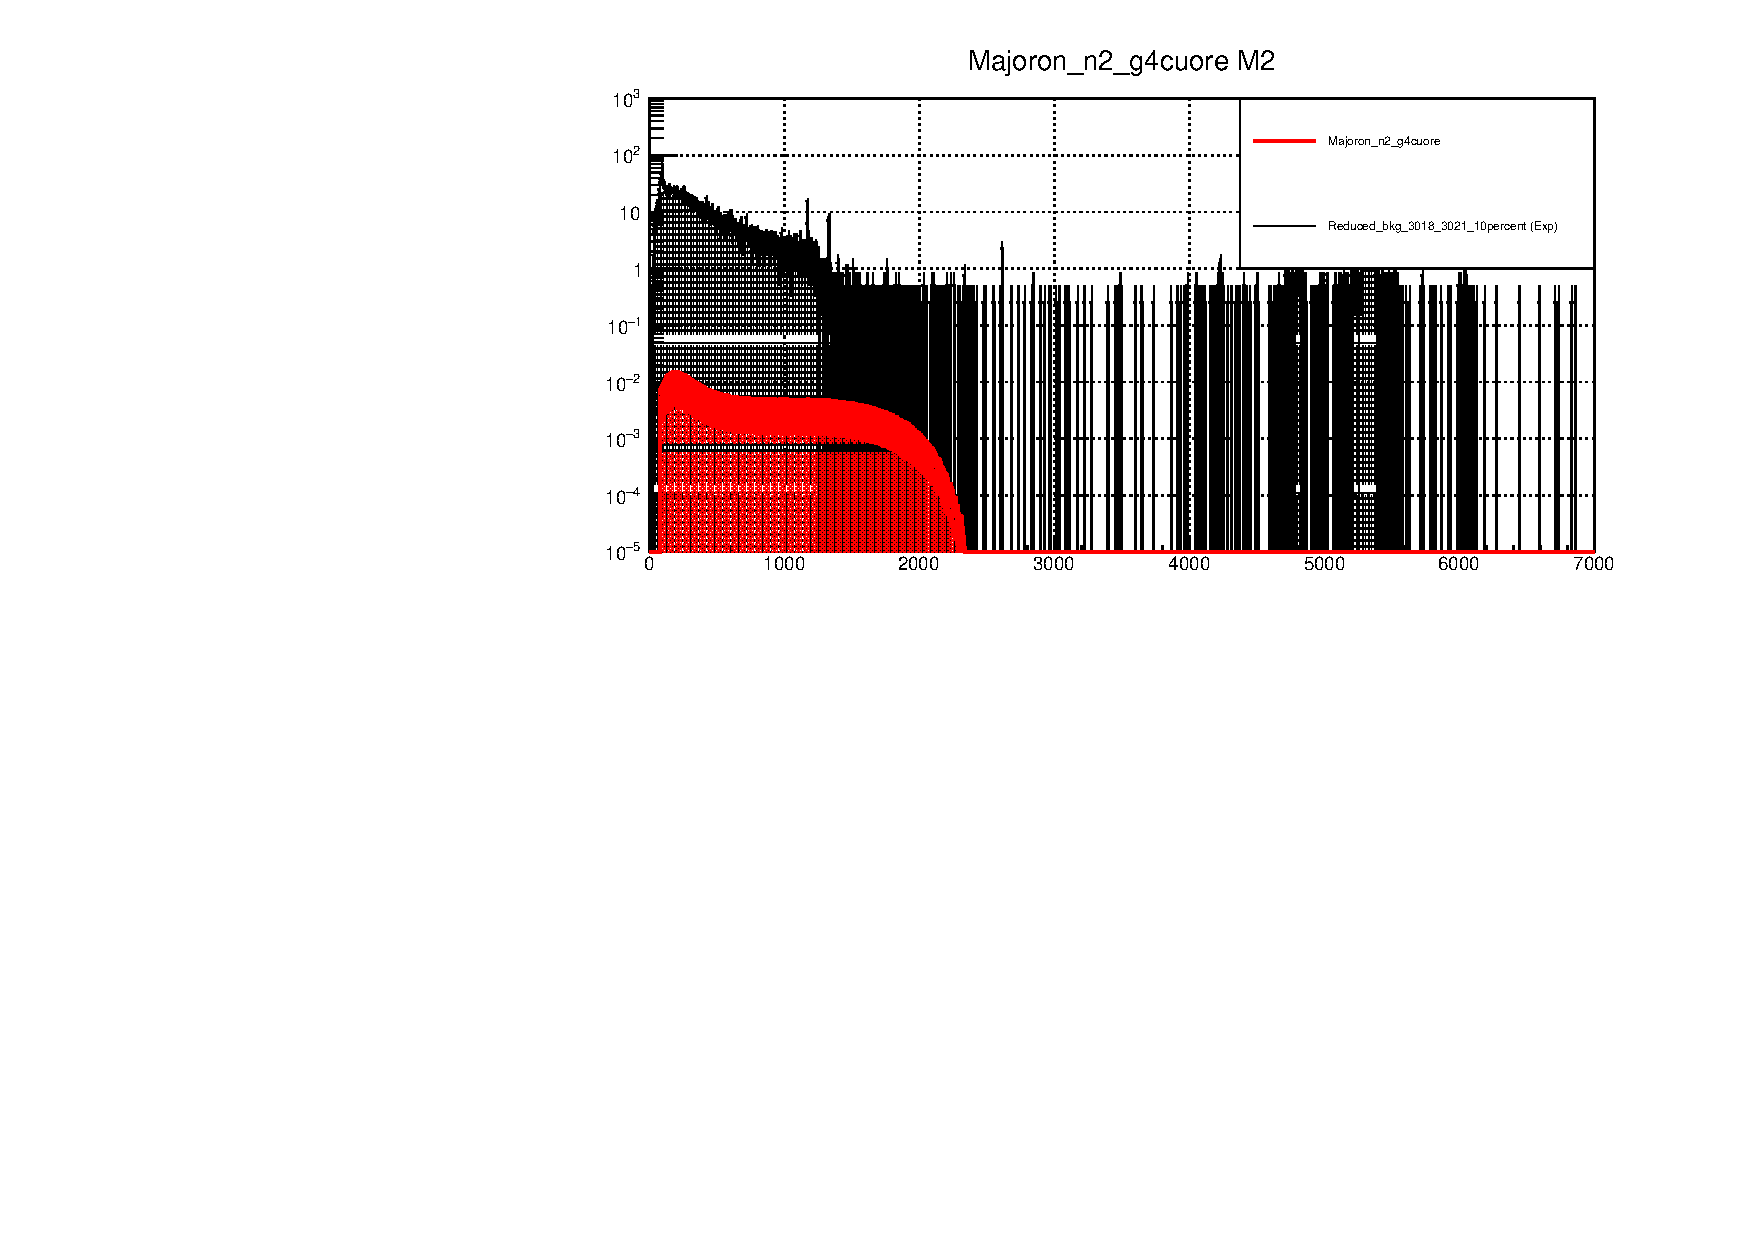
\includegraphics[width=0.9\textwidth]{Figures/Majoron_n2_g4cuore_M2.pdf}
\end{subfigure}
\qquad
\begin{subfigure}[t]{0.8\linewidth}
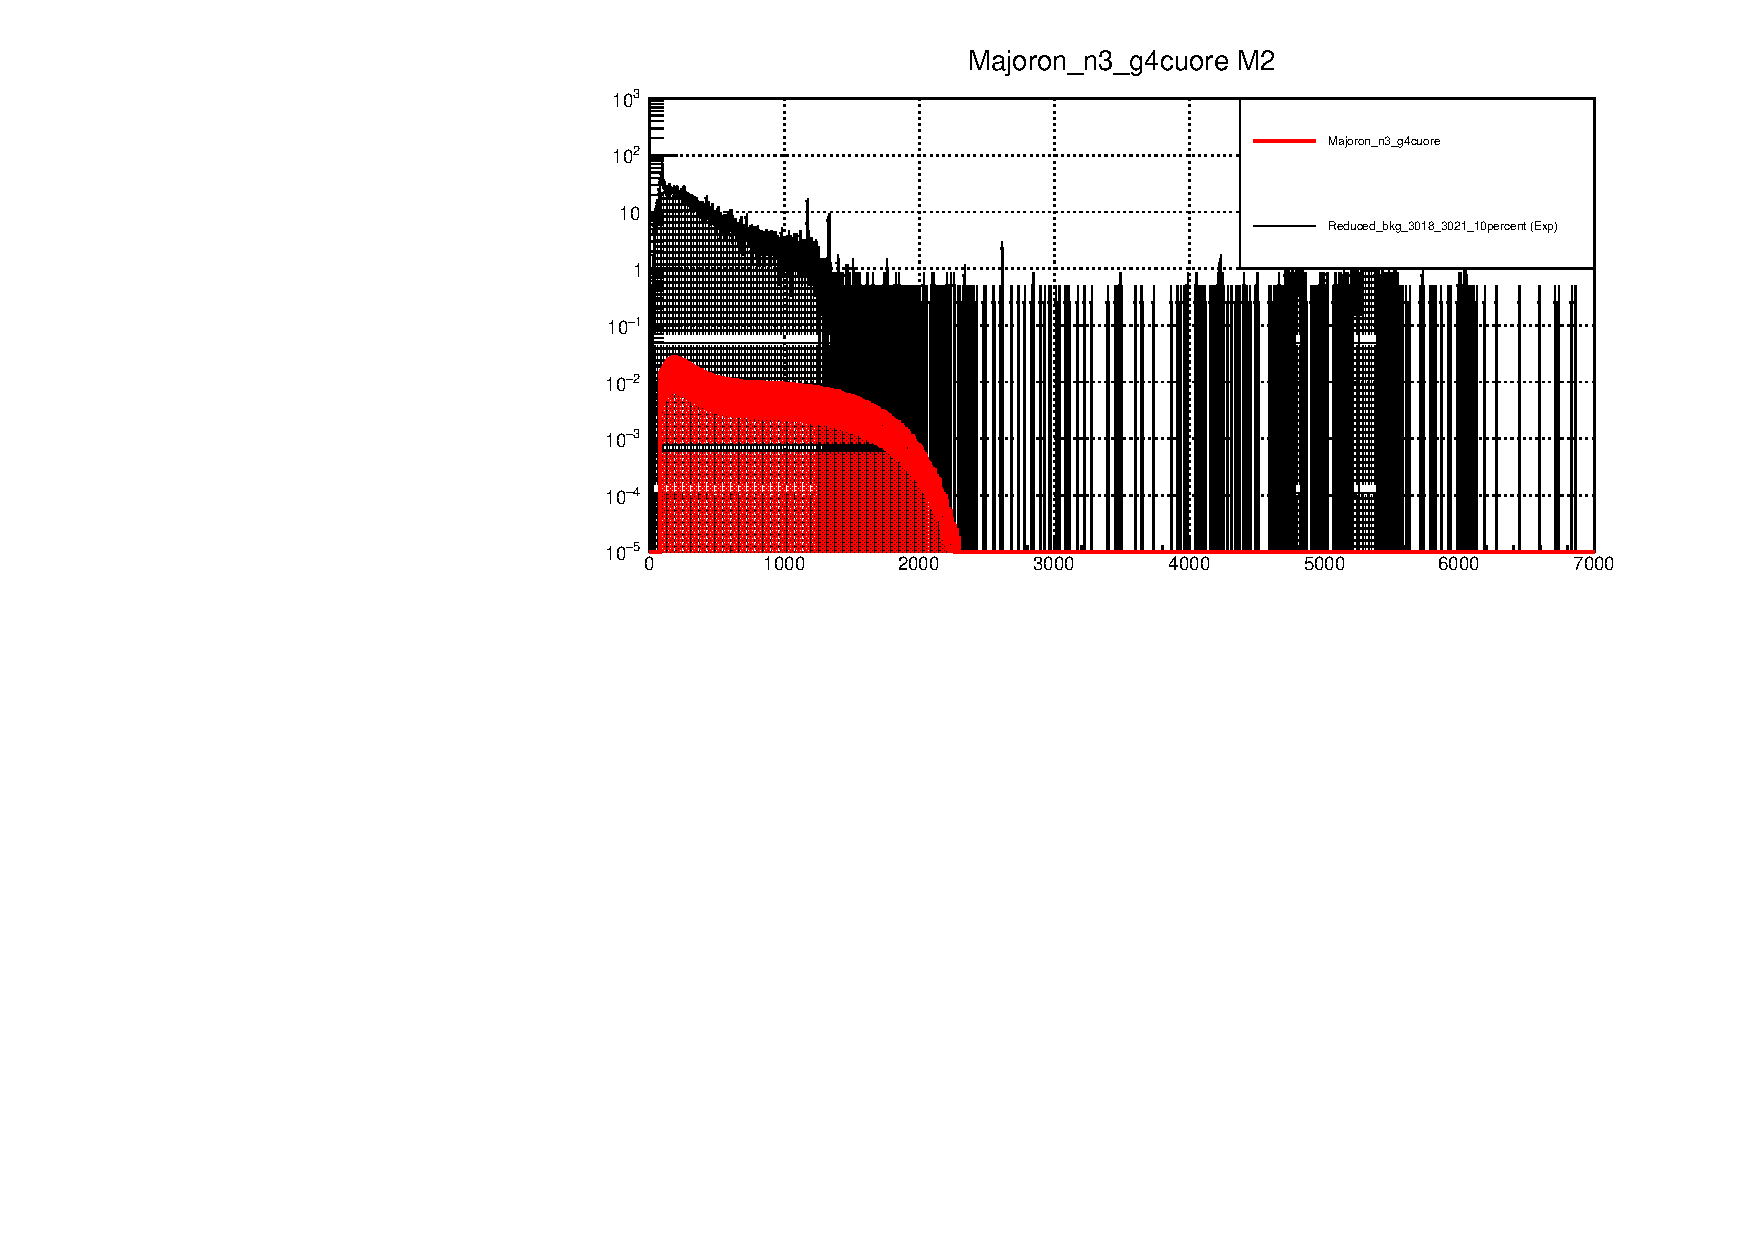
\includegraphics[width=0.9\textwidth]{Figures/Majoron_n3_g4cuore_M2.pdf}
\end{subfigure}
\qquad
\begin{subfigure}[t]{0.8\linewidth}
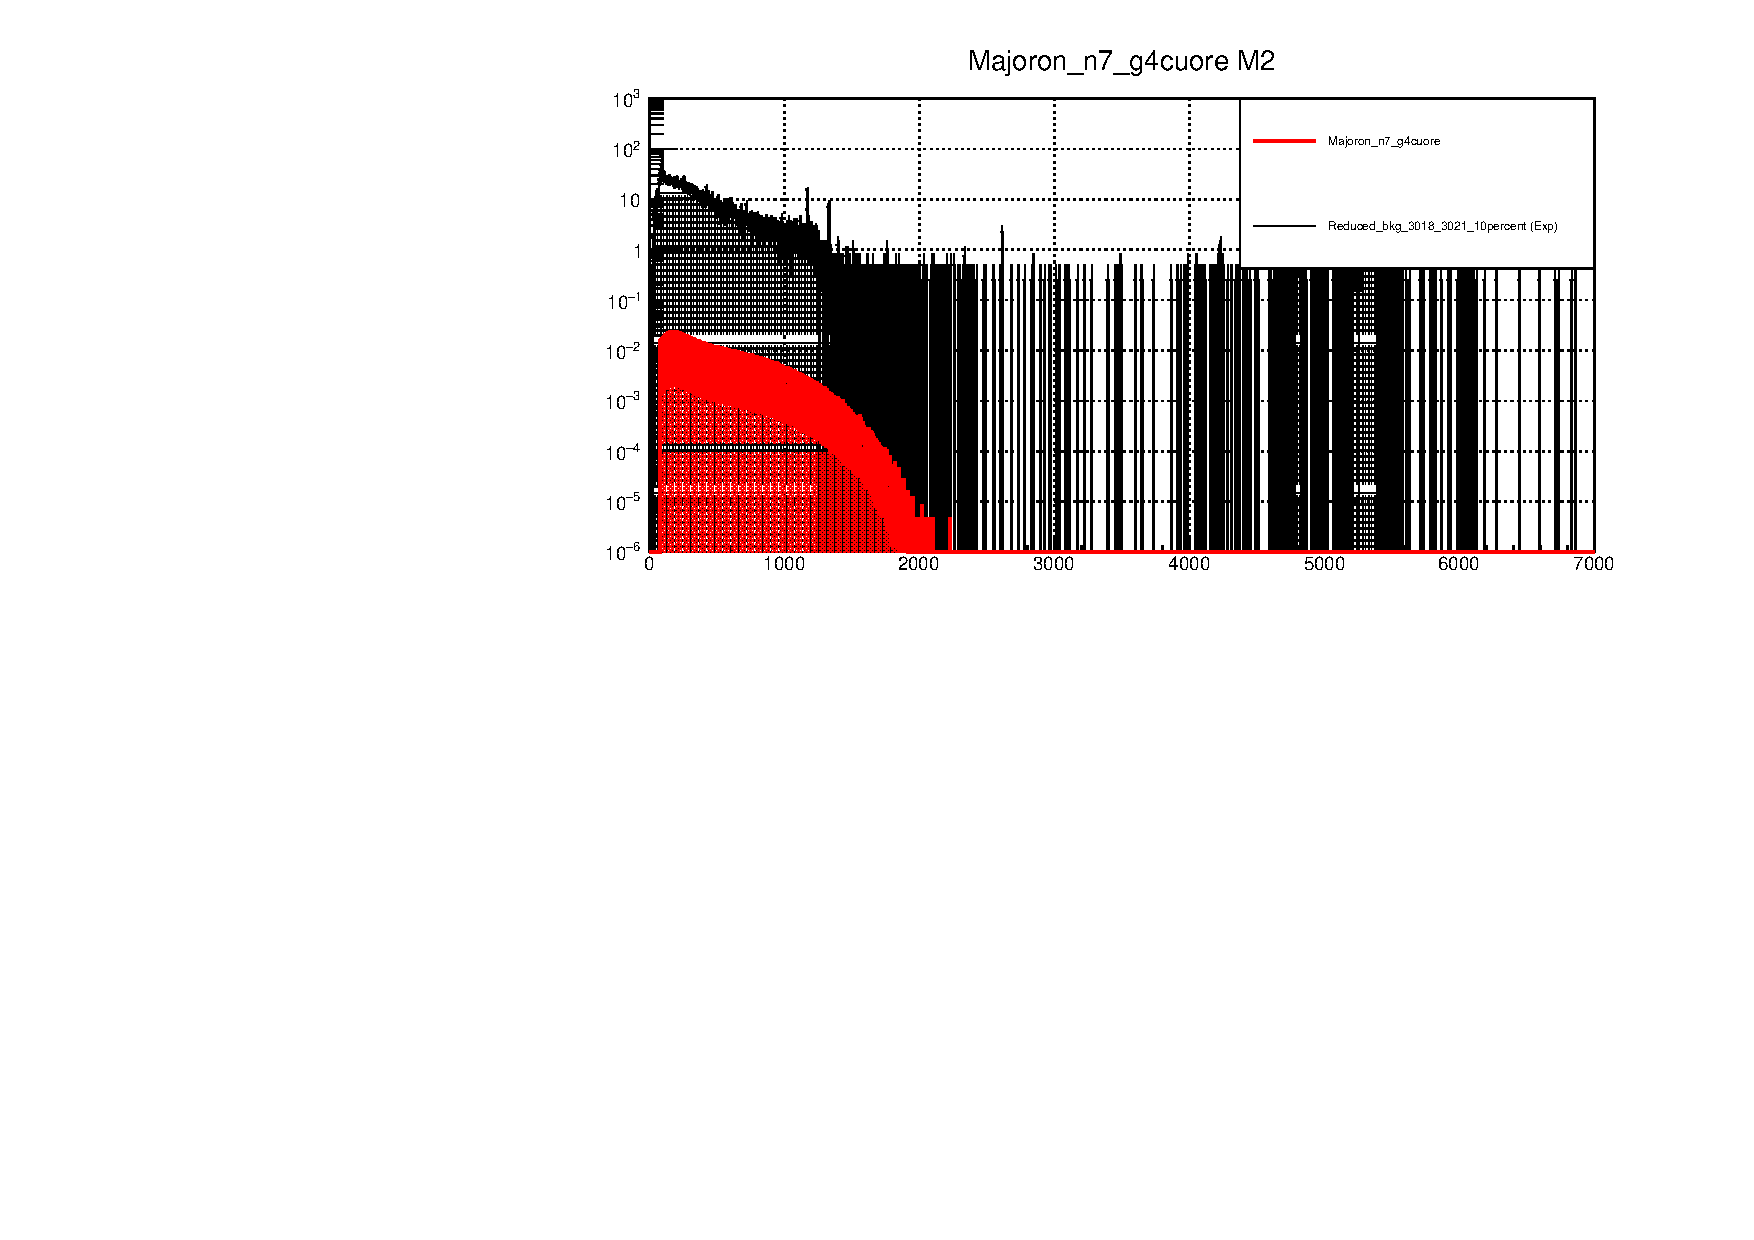
\includegraphics[width=0.9\textwidth]{Figures/Majoron_n7_g4cuore_M2.pdf}
\end{subfigure}
\caption[The fitted contribution of Majoron decays for the different spectral indices in the \Mtwo~ spectrum]{The fitted contribution of Majoron decays for the different spectral indices in the \Mtwo~ spectrum.}
\label{fig:SpectralIndicesM2Fit}
\end{figure}

Figures to include: Correlation matrix, Fit value distributions for all the Majoron spectra, background model with only 2nu -- describe deficiencies i.e. alpha region low-E and 2 MeV, systematics (floors, layers, etc.), 

\section{Majoron Systematics}
For the fits described above, it is important to also consider the systematics associated with each result.
Luckily, the set of systematics is similar for each of the 4 spectra, and are as follows:
\begin{description}[align=left]
\item [Geometric cuts] These include cuts on the data to only include specific parts of the detectors.
As the rate of Majoron decays should be independent of whatever geometric slice is included, testing this systematic quantifies the effect of other space-based asymmetries such as those shown in \autoref{fig:k40_towerfloors} that are not yet accounted for in the fit. 
\item[Analysis thresholds] The JAGS fit is performed with an analysis threshold set to 350 keV, but the fit should also be stable as the threshold is set to higher energies.
\item [Dataset-based cuts] Similarly to the geometric cuts, dataset-based cuts measure the effect of asymmetries in time or other effects due to changing conditions in the cryostat or analysis.
\item [Choice of priors] The priors chosen in the analysis are all uniform, non-informative priors, but it is important to quantify how these choices affect the result for a Majoron search.
In particular, the choices for priors on the sources that anticorrelate with a Majoron source, namely the \twonubb~and $^{147}$Sm decays, have strong affects on the measured value of the Majoron half-lives.
These priors are tested by taking the posterior values given from the $H_0$ fit and applied as the priors to the $H_1$ fit.
This answers a different question than the systematic choices listed above, and determines whether the $H_1$ fit truly improves the fit to the data or is merely a result of anticorrelations with multiple spectra.
The best-fit values for each of these systematics are shown in \color{red}add reference to plot here\color{black} and the 90\% upper limits on the half life are shown in \color{red}add reference to table here\color{black}.
\item [Fit Systematics] As thinning the MCMC can reduce the effect of bias, a longer chain with a larger $k$ picked for thinning can help estimate this autocorrelation bias in the fit.
If the choice of $k$ is already sufficient, this should have a negligible effect on the final result.

Figures to include:
Plot for best-fits for half-life (or normalization constant, haven't 100\% committed to either. Both are effectively the same), table of 90\% limits, table of fit references (e.g. floors, no Sm, etc.)
\end{description}
